\apendice

%Neste capítulo estão expostos os riscos previstos para o projeto.

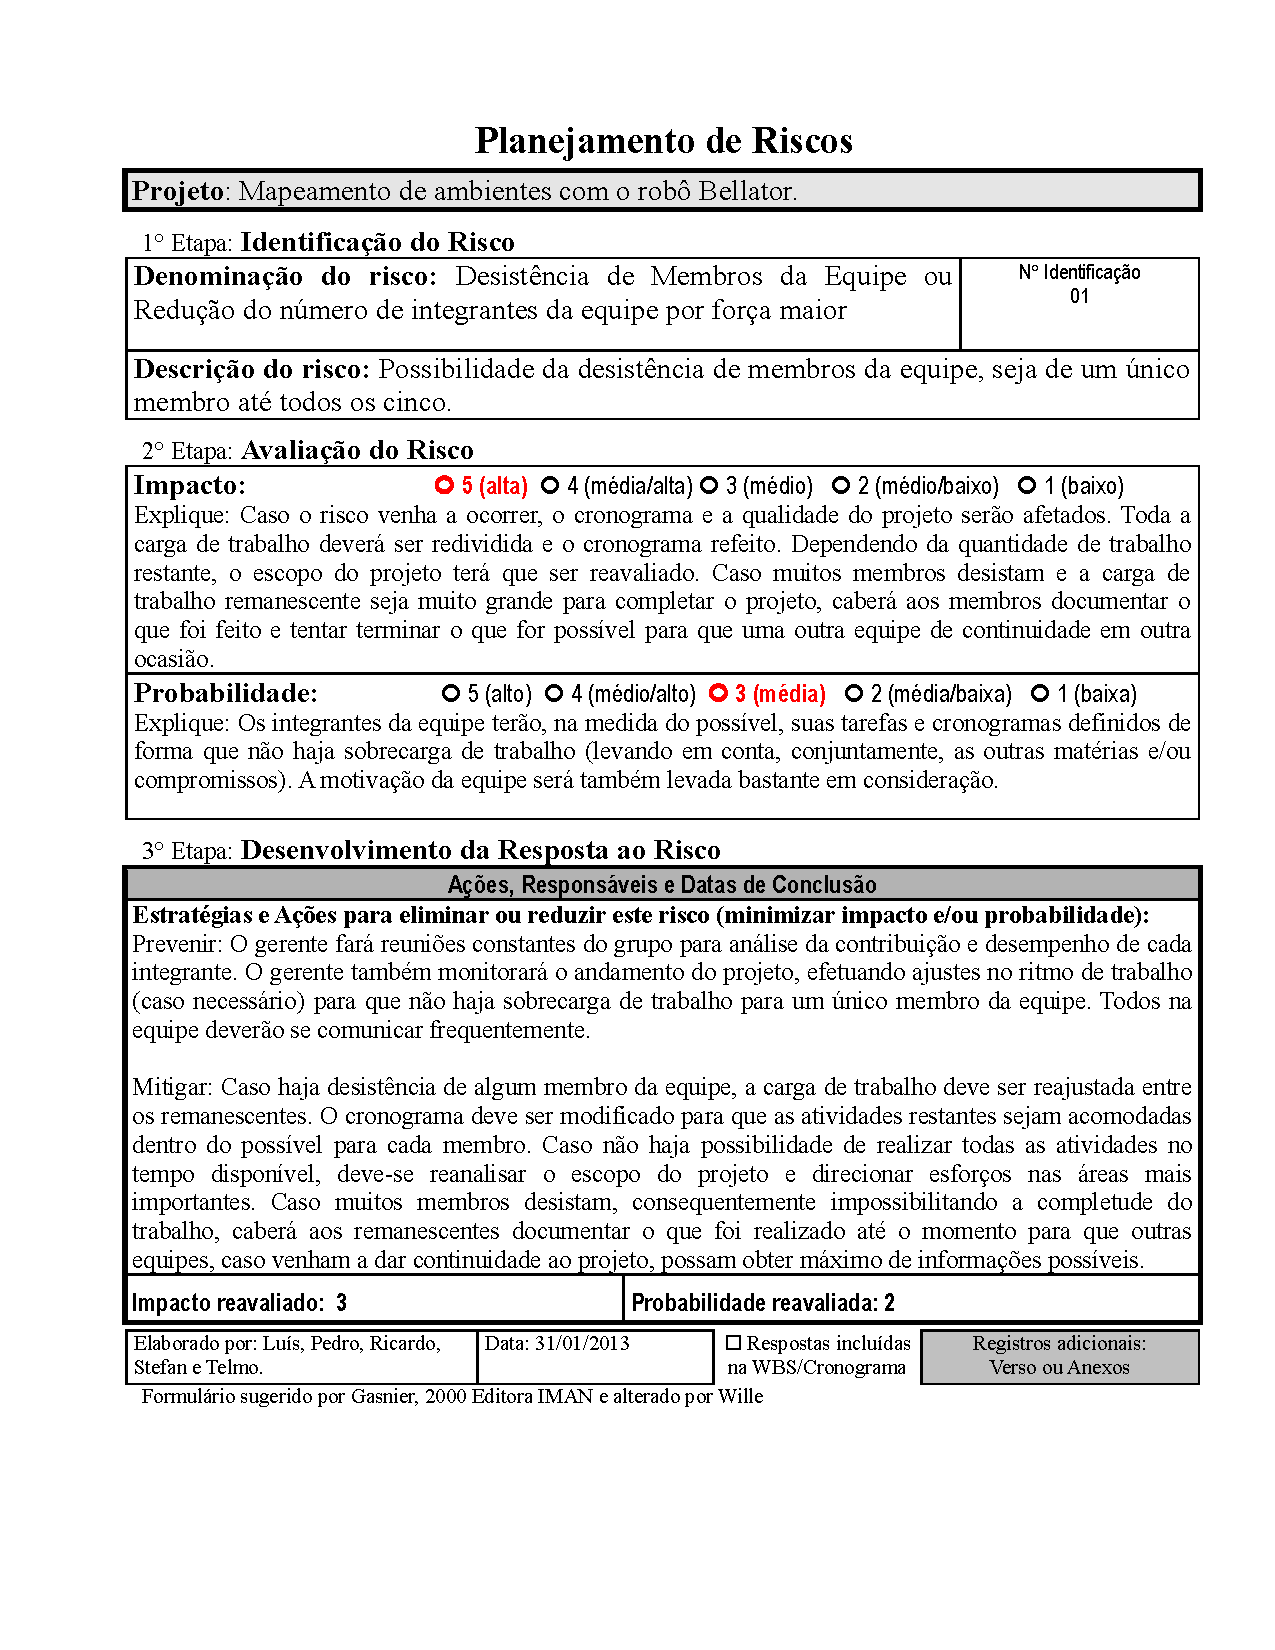
\includepdf[pages=1,scale=0.5, pagecommand=\chapter{Planejamento de riscos}]{Planejamento_de_Riscos_v3.pdf}
\includepdf[pages=2-9, pagecommand=]{Planejamento_de_Riscos_v3.pdf}


\chapter{Medidas do robô}
\label{cap:medidas_robo}
% Na Tabela \ref{tab:medidas_robo} estão presentes as medidas do robô.

\begin{table}[H]
  \caption{Medidas do robô.}
  \centering
  \begin{tabular}{l|l}
    \toprule
    \textbf{Medida} & \textbf{Valor} \\
    \midrule
    Comprimento da carcaça & 50 cm \\ \hline
    Largura da carcaça & 40 cm \\ \hline
    Distância entre a parte da frente do robô e os eixos das rodas & 14 cm \\ \hline
    Largura de cada roda & 4 cm \\ \hline
    Circunferência de cada roda & 64 cm \\ \hline
    Circunferência do eixo de cada roda & 7,5 cm \\ \hline
    Circunferência do eixo de cada encoder & 22 cm \\ 
    \bottomrule
  \end{tabular}
  \label{tab:medidas_robo}
\end{table}

\chapter{Diagramas detalhados de hardware}
\section{Diagrama elétrico/eletrônico}

Na figura \ref{fig:diagrama_eletrico_eletronico} mostra-se o diagrama de elétrico eletrônico do sistema embarcado. Cada bloco da figura \ref{fig:diagrama_blocos_hardware} corresponde a alguns componentes do diagrama elétrico eletrônico. A seguir detalha-se um pouco mais cada bloco.

\begin{figure}[H]
  \centering
  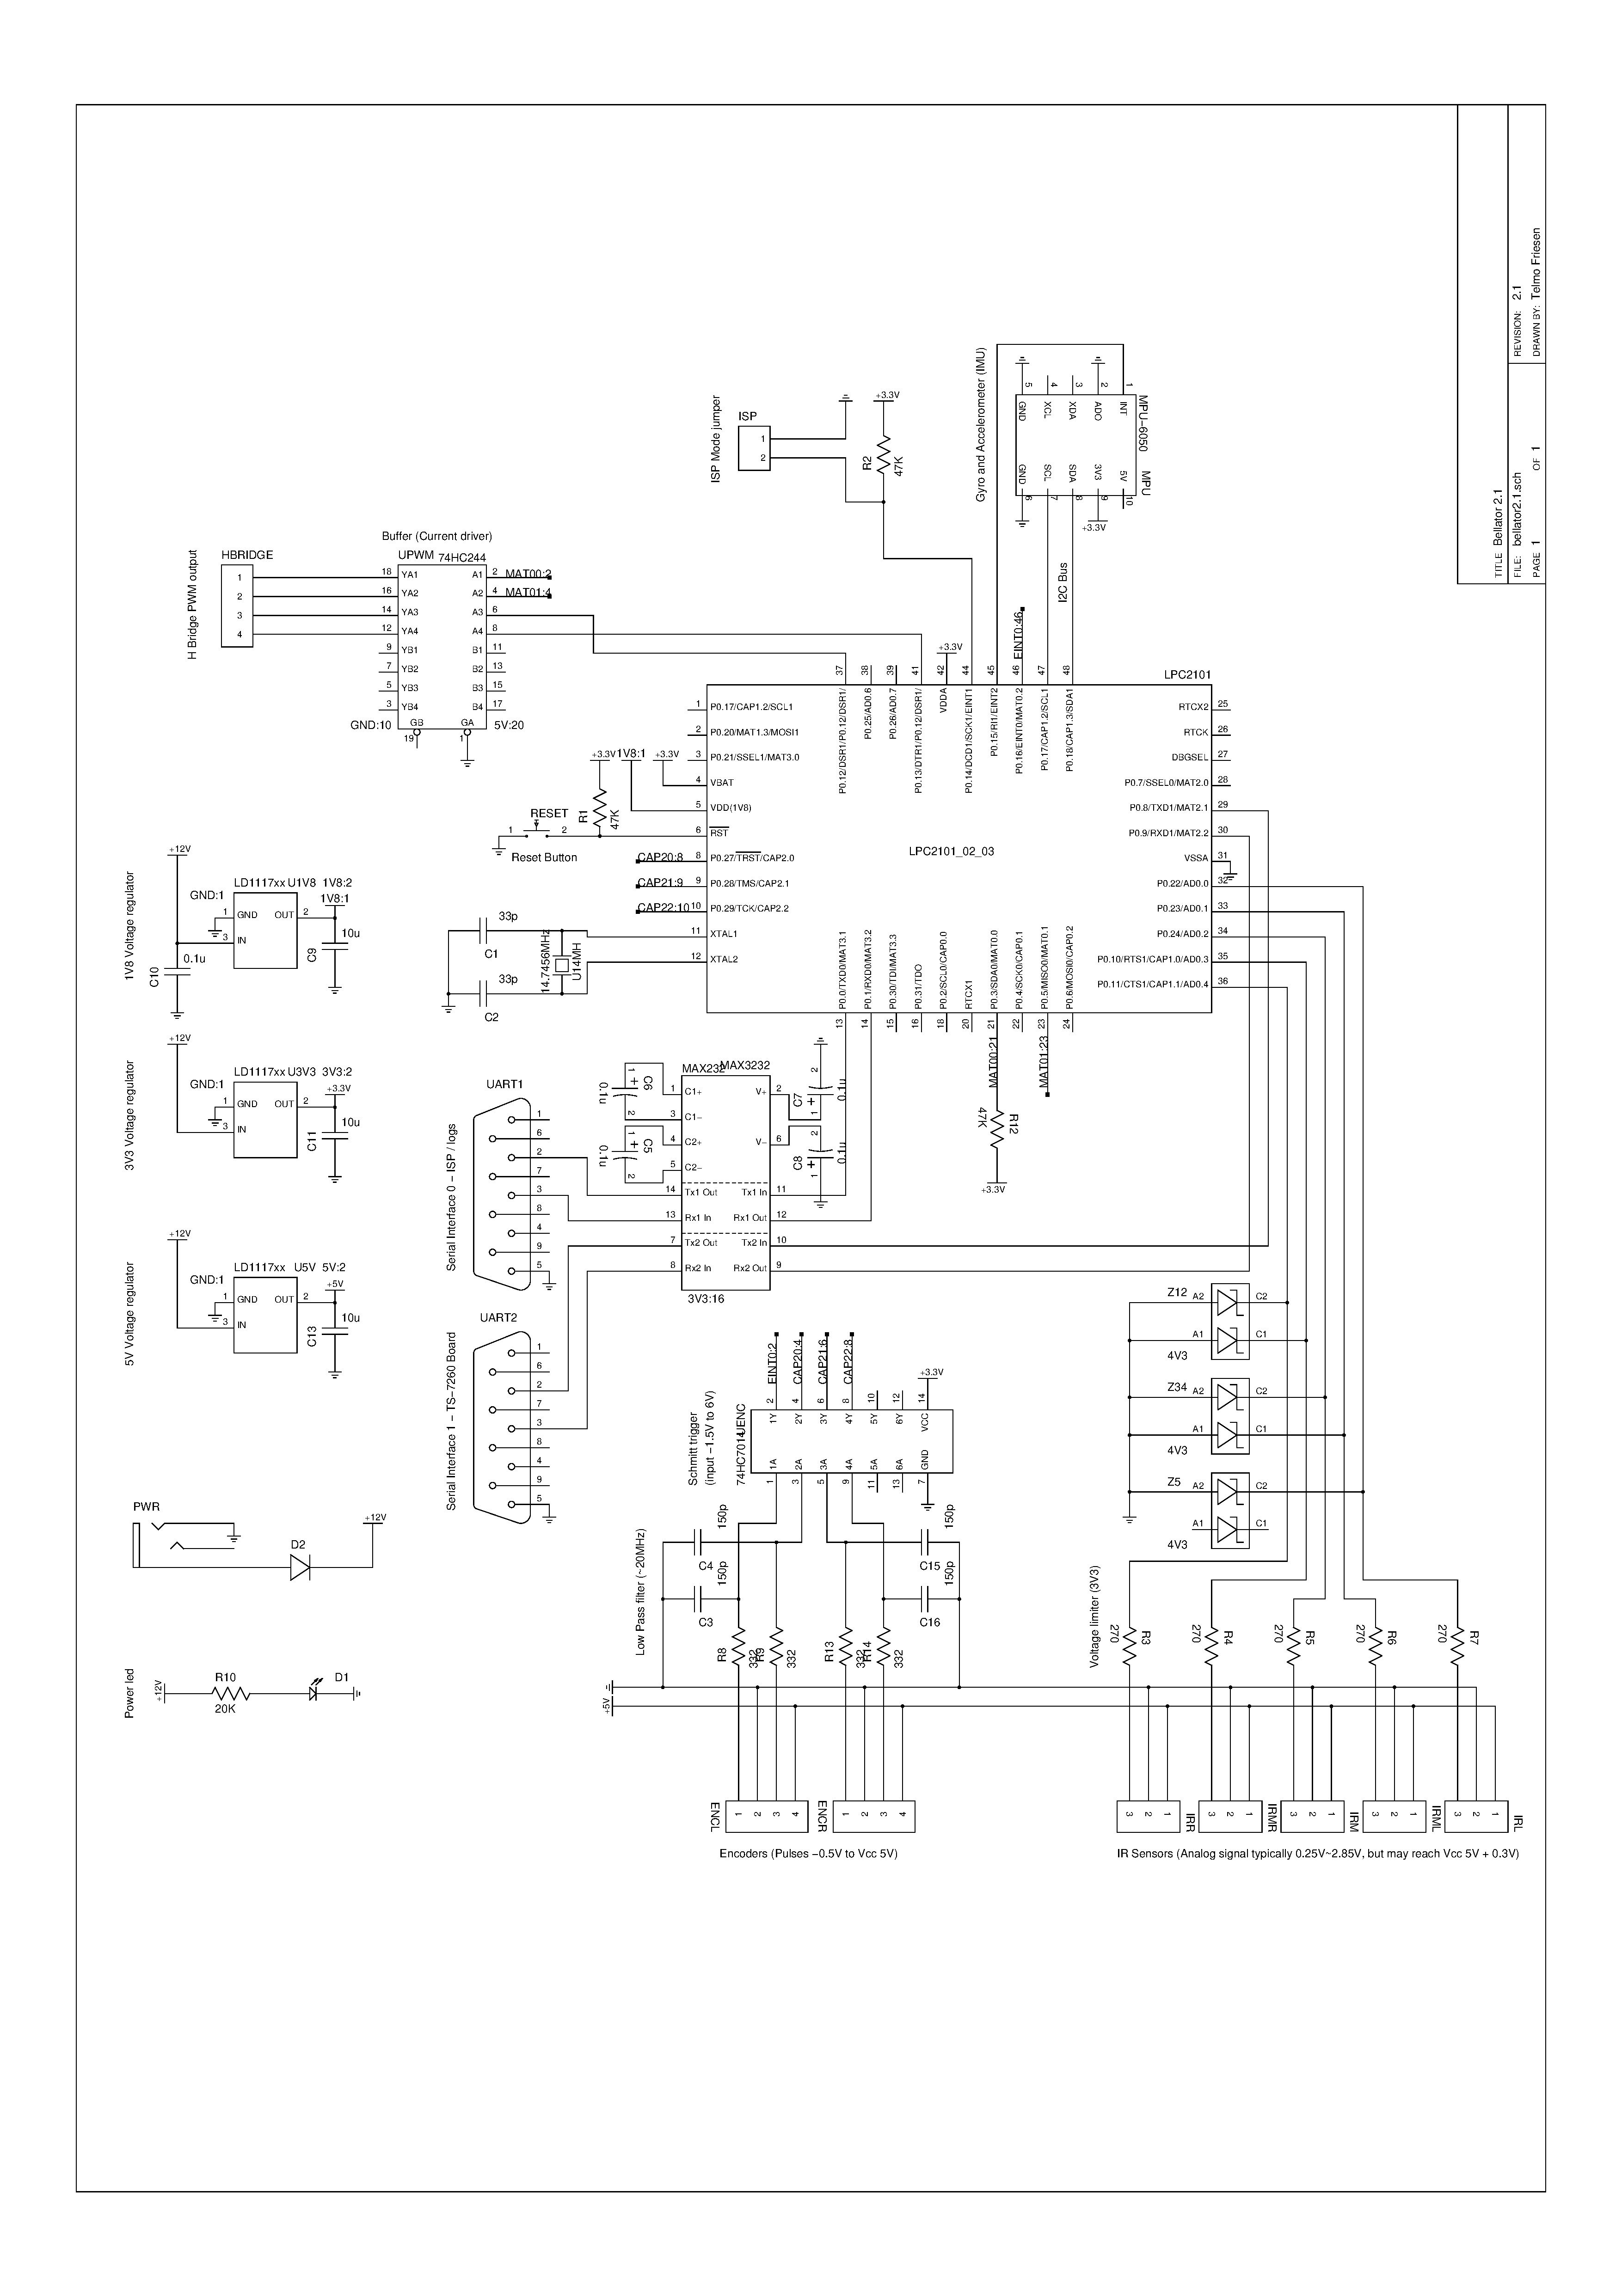
\includegraphics[width=0.9\textwidth, keepaspectratio]{./figuras/hardware/hardware2_2.pdf}
  \caption{Diagrama elétrico/eletrônico.}
  \label{fig:diagrama_eletrico_eletronico}
\end{figure}

\begin{enumerate}[topsep=0pt, partopsep=0pt, itemsep=0pt]
    \item Microcontrolador: Composto pelo microcontrolador LCP2103 da NXP que possui arquitetura ARM. Ele dispõe de duas interfaces seriais, conversor analógico digital com 8 canais, interface i2c, entradas de captura e interrupção, saídas de PWM entre outras funções que não serão utilizadas nesse projeto.
    \item UART 0/1: Constituído por um chip max3232 que opera em níveis de tensão CMOS e que gera os níveis adequados para o padrão RS-232 utilizando alguns capacitores.
    \item Buffer: Constituído por um chip 74HC244, é responsável por fornecer corrente e elevar os níveis de tensão de saída do microcontrolador de 3,3V para 5,0V.
    \item IMU: Composto pela placa de desenvolvimento MPU-6050, que possui um chip com o mesmo nome, MPU-6050, e circuitos RC auxiliares necessários para o funcionamento do MPU-6050.
    \item Limitador de tensão: Constituído de um resistor com baixo valor, 270 ohms, e um diodo Zener polarizado reversamente e com tensão de ruptura de 4.3V. Quando a tensão de entrada ultrapassar 4.3V o diodo passa a conduzir e mantém a tensão de 4.3V no resistor. O datasheet do microcontrolador sugere que se mantenha a impedância da carga menor que 40kohms, logo a adição de um resistor de 270 ohms pode ser desconsiderado com relação ao erro que possa causar na leitura do conversor. Um resistor de 270 ohms leva a uma corrente de 3.7mA quando a saída do sensor for 5.3V, que é o valor máximo previsto no datasheet.
    \item Tratamento de sinal: Composto por um filtro RC passa baixas e um chip 74HC7014. As frequências acima de 20MHz são atenuadas no sinal do encoder. Esse valor foi calculado com base na forma de onda da saída especificada no datasheet do encoder. Para tanto utilizam-se resistores de 332 ohms e capacitores de 150pF.
\end{enumerate}


\section{Placa de circuito impresso}

O projeto da placa de circuito impresso (PCB) do sistema embarcado de baixo nível está explicitado nas Figuras \ref{fig:pcb_cima} e \ref{fig:pcb_baixo}. Na Figura \ref{fig:pcb_pronta} está presente uma foto da placa pronta com os componentes soldados.

\begin{figure}[H]
  \centering
  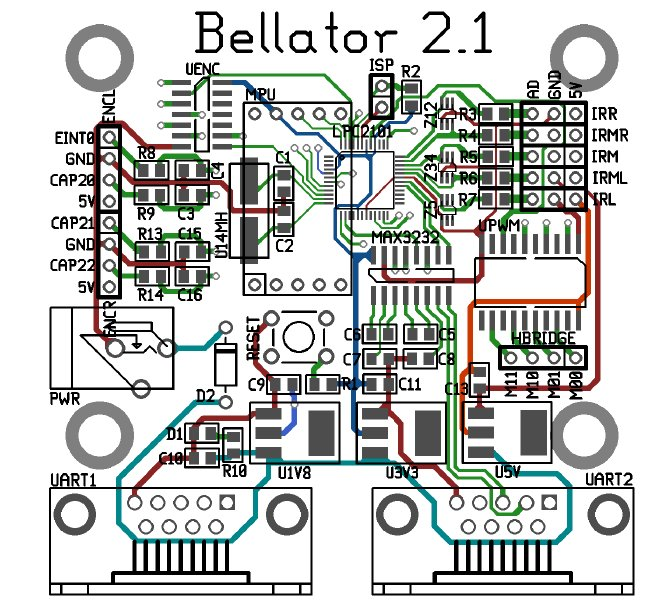
\includegraphics[width=0.7\textwidth, keepaspectratio]{./figuras/hardware/pcb_cima.jpg}
  \caption{Projeto da PCB -- lado de cima.}
  \label{fig:pcb_cima}
\end{figure}

\begin{figure}[H]
  \centering
  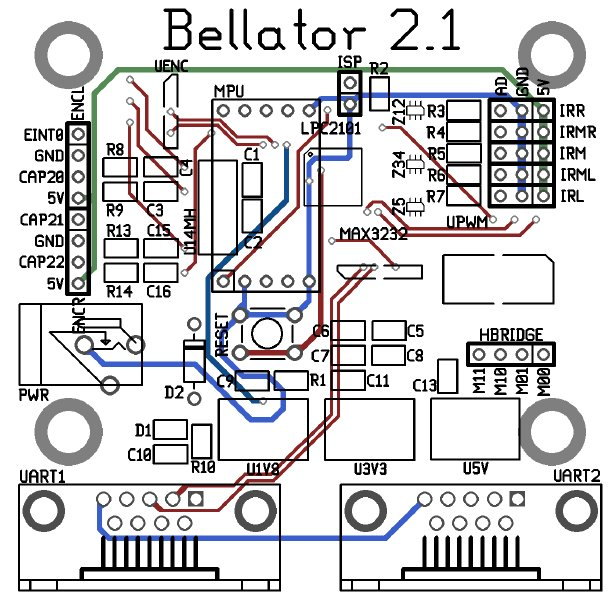
\includegraphics[width=0.7\textwidth, keepaspectratio]{./figuras/hardware/pcb_baixo.jpg}
  \caption{Projeto da PCB -- lado de baixo.}
  \label{fig:pcb_baixo}
\end{figure}

\begin{figure}[H]
  \centering
  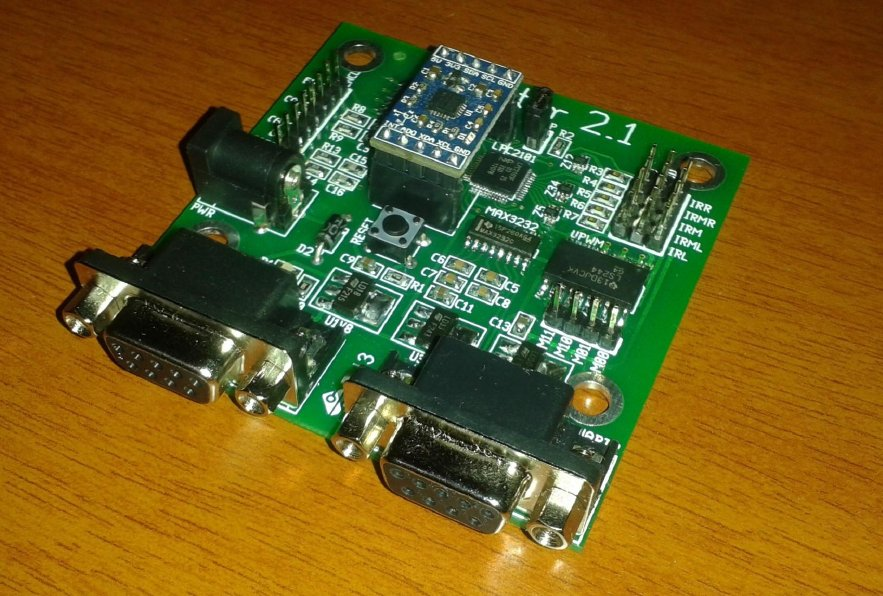
\includegraphics[width=0.7\textwidth, keepaspectratio]{./figuras/hardware/pcb_pronta.jpg}
  \caption{PCB montada.}
  \label{fig:pcb_pronta}
\end{figure}

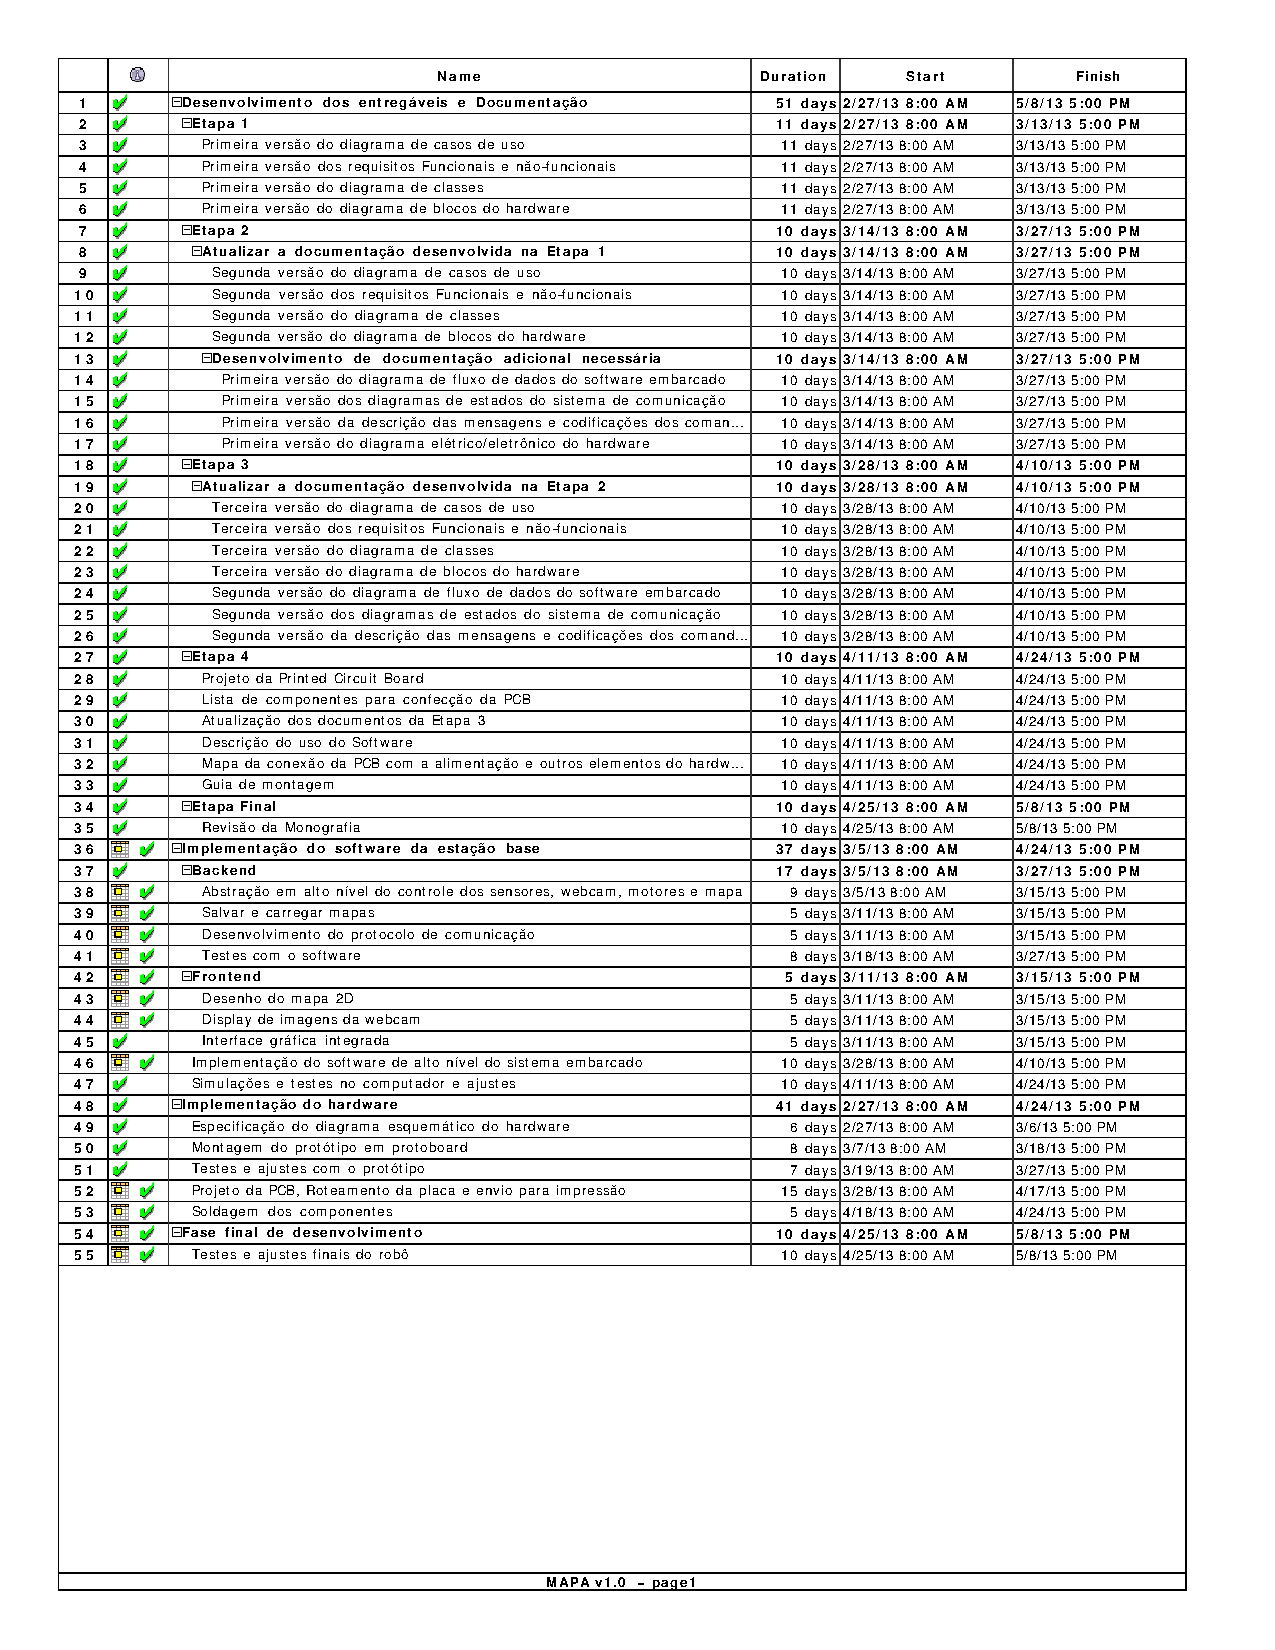
\includepdf[pages=1,offset=0 -130, pagecommand=\chapter{Cronograma}]{cronograma.pdf}

\raggedright